%%
%%  appendixPolarCalib.tex - Obstacle Detection and Planning for Autonomous Vehicles based on Computer Vision Techniques
%%
%%  Copyright 2014 Néstor Morales <nestor@isaatc.ull.es>
%%
%%  This work is licensed under a Creative Commons Attribution 4.0 International License.
%%

\graphicspath{{./images/chapter04/bmps/}{./images/chapter04/vects/}{./images/chapter04/}}

\chapter{Polar Rectification}\label{ch:appendix_polar_calib}

In chapter \ref{ch:chapter04}, we registered a pair of images obtained between frames, with the aim of distinguishing real from fake obstacles. The best way to do such a registration is through a polar rectification process \citep{pollefeys1999simple}. This non-linear polar rectification method allows registering the images along the time, helping in the detection of motion. The basis of this method is to reparameterize the images by setting the coordinates of their pixels in terms of the epipoles of a stereo pair. In this process, a linear transformation has to be found for every wedge part of the image with vertex at the epipole. This allows rectifying the whole image for every possible epipolar configuration, while keeping the size of resulting image reasonably large. The algorithm is designed in such way that no pixel loss is guaranteed. Also the length of original epipolar lines is preserved. The resulting image is upper-bounded by a size of $(2 (W + H) \times \sqrt{W^2 + H^2})$, where $W$ is the image width and $H$ its height. An implementation of this method is made available at \url{https://github.com/nestormh/PolarCalibration}.

In order to reduce the matching ambiguity to a half of the epipolar line in a case of epipole inside the image, it uses the concept of oriented epipolar geometry. To do this, one point correspondence is needed in both views. With this information, just positive coordinates over the epipolar line will be taken into account. The transfer of corresponding epipolar lines is obtained from the expression:

\begin{equation}\label{eq:cp04_epipolar_lines}
l_{t - 1} \sim H^{-T}l_t\text{, or }l_t \sim H^T l_{t - 1}
\end{equation}

Here, $l'$ is the epipolar line at image at frame $t$, and $l$ the corresponding epipolar line at frame $t - 1$. $H$ is an homography for an arbitrary plane, which can be obtained from the fundamental matrix $F$ \citep{luong1996fundamental}:

\begin{equation}\label{eq:cp04_homography}
H = [e_{t - 1}] \times F + e_{t - 1}^T a
\end{equation}

, where $a$ is a random vector for which $det(H) \neq 0$, so that $H$ is invertible. $e$ is the epipole.

The first step in the polar rectification process consists on the definition of the common region between both images. To do that, we first need to compute the epipoles for both images and the homography $H$. So we need to know first the fundamental matrix $F$. The epipolar geometry is described by the following equation:

\begin{equation}\label{eq:cp04_fundamental_matrix}
m_{L,t - 1}^T \cdot F \cdot m_{L,t}= 0
\end{equation}

, where $m_{L,t - 1}$ and $m_{L,t}$ are homogenous representations of corresponding image points in the left image of the frames $t$ and $t - 1$, respectively. So we need to compute these matches. To ensure that we just get correct matches, we compute the correspondences between image pairs in the following order: $I_{L, t} \rightarrow I_{R, t} \rightarrow I_{R, t - 1} \rightarrow I_{L, t - 1} \rightarrow I_{L, t}$, where $I_{\{L,R\},t}$ is the left ($L$) or right ($R$) image at frame $t$. From a initial set of features in $I_{L, t}$, we get the valid matches in $I_{R, t}$, and the cycle is completed until we reach $I_{L, t}$ again, keeping just the valid matches. A match is valid if satisfies the following rules:
\begin{itemize}
 \item At the end of the cycle, points obtained should be the same as those from which we started the process. If not, a wrong match was found in the way.
 \item Features in $I_{L, t}$ must be in the same row as $I_{R, t}$. As images are rectified, the vertical component should be the same. Same applies to $I_{L, t - 1}$ and $I_{R, t - 1}$.
 \item The 2D distance between features from frame $t$ and $t - 1$ should not be too big, since the frame rate is high and images do not change too much between frames.
\end{itemize}

The result of this matching process is represented at figure \ref{fig:cp04_polar_fund_matrix_computation}. There, each matching cycle is represented by the same random color.
\begin{figure*}[h!]
\centering
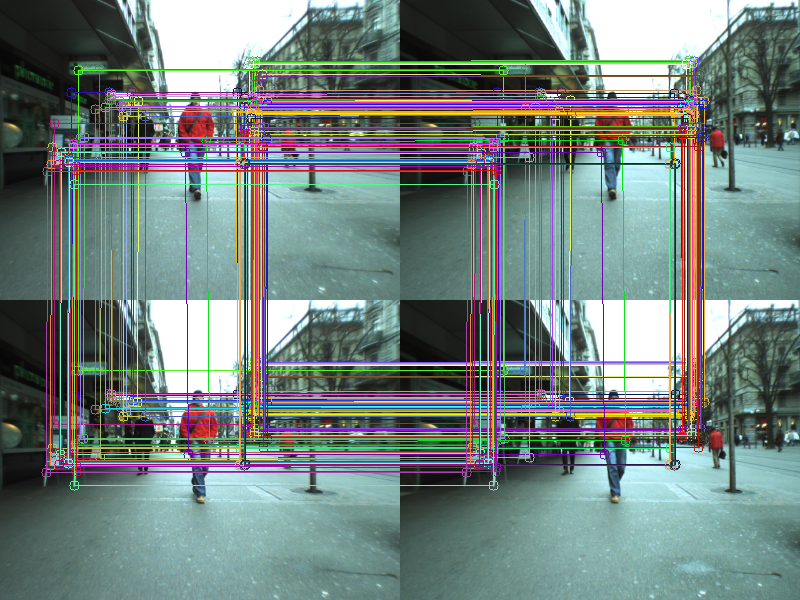
\includegraphics{fundamentalMatrixComputation}
\captionof{figure}{Looking for the common points in frames $t$ and $t - 1$.}\label{fig:cp04_polar_fund_matrix_computation}
\end{figure*}

Once we get these matches, we solve the system described by equation \ref{eq:cp04_fundamental_matrix}, obtaining $F$. From $F$, it is possible to get also the homography $H$ and the epipoles $e_t$ and $e_{t-1}$. So we can start looking for the common region between the images. This common region will be determined by the extremal epipolar lines, which will be those that touch the outer image corners. We must deal with three possible cases depending on
whether the epipoles are located inside or outside the image. These three cases are shown at figure \ref{fig:cp04_polar_common_region}.

\begin{figure}[h!]
\centering

\includegraphics[width=0.8\textwidth]{polar_common_region}
\captionof{figure}{The three possible cases depending on the position of the epipoles.}\label{fig:cp04_polar_common_region}
\end{figure}

There, $I_i^j$ refer to the extremal lines for each image, where $i$ indicates if it is the current ($t$) or the previous ($t - 1$) image, and $j$ is the corner with which the line intersects (1 and 2 for the current image and 3 and 4 for the previous one), so $I_i^j = [e_i] \times c_j$. If the epipole is located inside the image we need to decide which half-epipolar lines, pointing in oposite direction, is the correct one.


\begin{figure}[h!]
\centering
\begin{tabular}{cc}
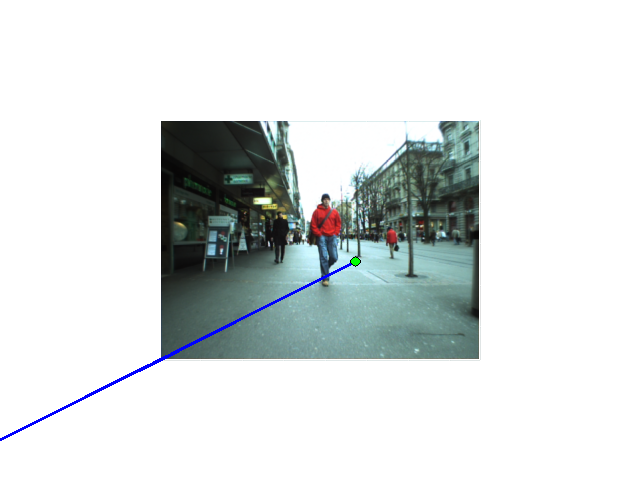
\includegraphics[width=0.40\textwidth]{epipolarExtremeLeft1}\label{fig:cp04_epipolarExtremeLeft1} &
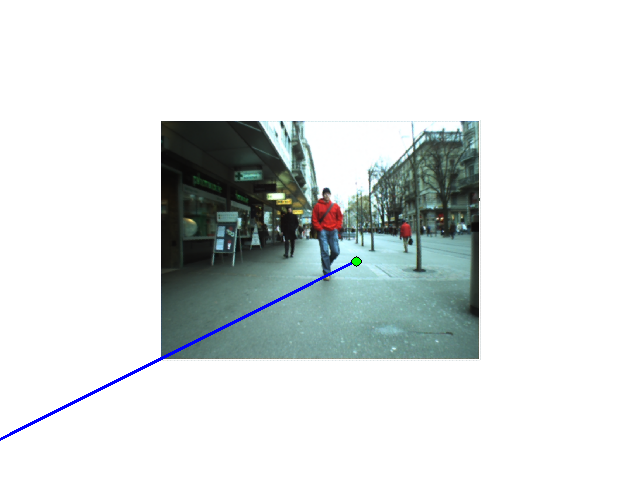
\includegraphics[width=0.40\textwidth]{epipolarExtremeRight1}\label{fig:cp04_epipolarExtremeRight1} \\
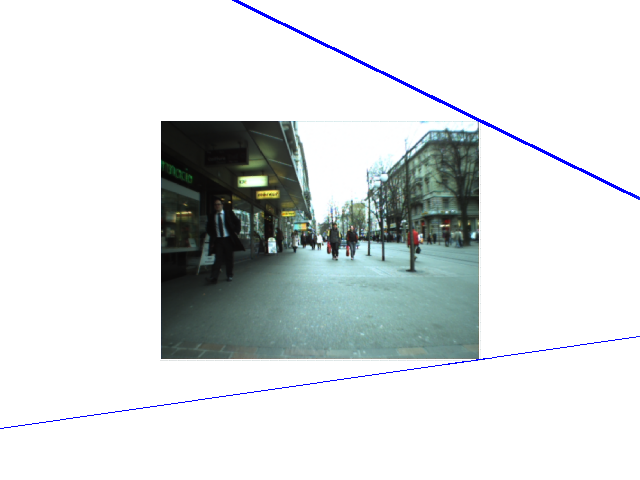
\includegraphics[width=0.40\textwidth]{epipolarExtremeLeft2}\label{fig:cp04_epipolarExtremeLeft2} &
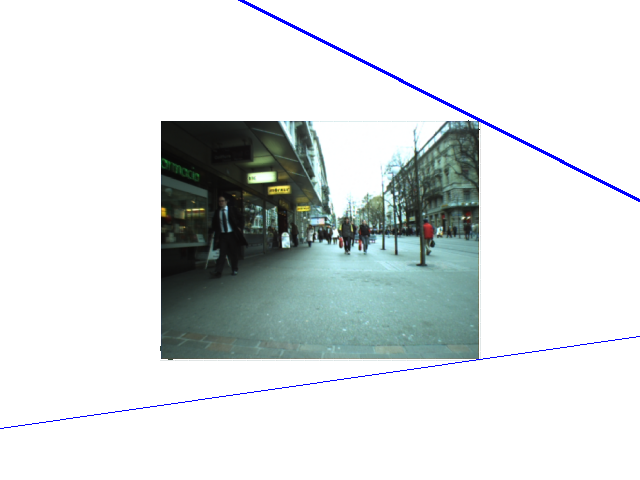
\includegraphics[width=0.40\textwidth]{epipolarExtremeRight2}\label{fig:cp04_epipolarExtremeRight2} \\
\end{tabular}
\captionof{figure}{Two examples of the external epipolar lines found for a case in which the epipole is inside the image for both images (top row); and out, also in both images (bottom row).}\label{fig:cp04_epipolarExtreme}
\end{figure}

\FloatBarrier

In image \ref{fig:cp04_epipolarExtreme}, two examples of the outer epipolar lines found are shown. From these, the common region is defined, which will be represented by the beginning and ending epipolar lines $I_i^B$ and $I_i^E$. If both epipoles are inside the image, an arbitrary epipolar line can be used. In that case, we can avoid boundary effects by adding a small overlap. That is, we will use a region a little bit bigger than $360\textdegree$.

Then, starting from $I_i^B$, we start constructing the rectified image, line by line, until we reach the epipolar line $I_i^E$. This process is repeated for $i=t$ and $i=t-1$ so, at the end of it, we will have both images rectified. In these images, each of the rows will have a correspondence with a certain epipolar line. The distance between two consecutive epipolar lines is determined independently for each of the lines so we avoid pixel compression. The benefits of doing such non-linear warping are that this allows getting the smallest image without information loss.

\begin{figure}[h!]
    \centering
    \begin{tabular}{ cc }
      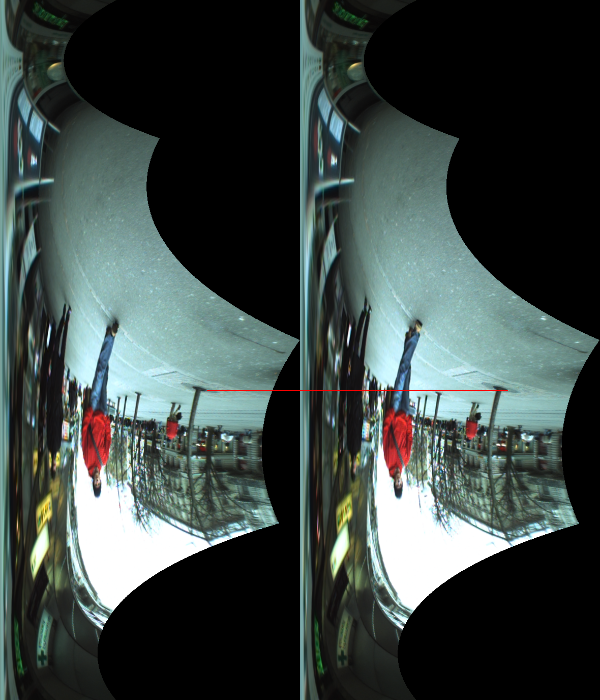
\includegraphics[width=0.4\textwidth]{polarRectification}\label{fig:cp04_polarRectification} &
      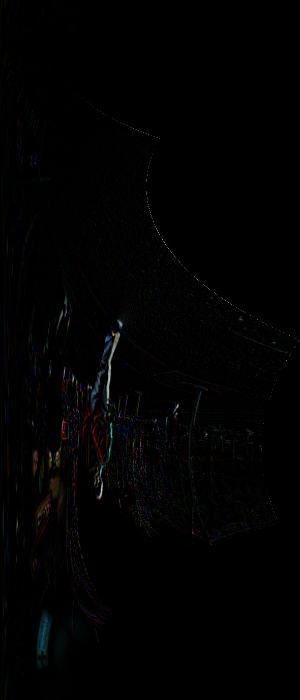
\includegraphics[width=0.2\textwidth]{polarDiff}\label{fig:cp04_polarDiff}
    \end{tabular}
  \caption{Example of a rectified pair of frames. Red line shows that the alignment is correct. On the right, the absolute difference of both rectified images is shown.}\label{fig:cp04_polarRectification_example}
\end{figure}

Using this method, we compute a transformation map that allows knowing the correspondences of the pixels of each image in euclidean and in polar coordinates easily and without a meaningful computational cost. With such a map, we compute a pair of images as those shown in the left side of figure \ref{fig:cp04_polarRectification_example}. Red line demonstrates that the alignment obtained is correct. 
